
\begin{center}
	{\scriptsize
		\begin{tabularx}{\textwidth}{p{0.2\textwidth}|p{0.6\textwidth}|p{0.1\textwidth}}
			\caption{Summary of methods for achieving the objectives} \label{tab:achieve_objective} \\
			\hline 
			\hline 
			\textbf{Objectives} & 
			\textbf{Methods} & 
			\textbf{Locations} \\ 
			\hline 
			\endfirsthead
			\multicolumn{3}{c}%
			{\textit{Continued from previous page}} \\
			\hline
			\hline 
			\textbf{Objectives} & 
			\textbf{Methods} & 
			\textbf{Locations} \\ 
			\hline 
			\endhead
			\hline 
			\multicolumn{3}{r}{\textit{Continued on next page}} \\ 
			\endfoot
			\hline 
			\endlastfoot
			\hline
			
			\Paste{GO} & 
			Expected Results:
			\begin{enumerate}
				\item Successfully developed a user-priority-based grading and sorting system using machine learning and computer vision which can assess the mangoes’ ripeness, size and bruises.
			\end{enumerate} 
			Actual Results:
			\begin{enumerate}
				\item More work needs to be done to fine tune the software components to achieve higher accuracy such as changing hyperparameters or using a newer version of EfficientNet
				\item More work needs to be done to make the hardware component more robust such as by fixing the camera and LED lights in place
			\end{enumerate} 
			& Sec.~\ref{sec:summary_results_and_discussions} on p.~\pageref{sec:summary_results_and_discussions} \\ \hline
			
			\Paste{SO1} & 
			Expected Results:
			\begin{enumerate}
				\item Successfully integrated a conveyor belt with the image acquisition in order to achieve efficient flow of automated sorting and grading of the mangoes.  
				\item Successfully integrated LED strips to provide optimal lighting for image capturing of the mangoes.
				\item Successfully fixed the hardware components in place
			\end{enumerate} 
			Actual Results:
			\begin{enumerate}
				\item Successfully integrated a conveyor belt with the image acquisition in order to achieve efficient flow of automated sorting and grading of the mangoes.  
				\item Successfully integrated LED strips to provide optimal lighting for image capturing of the mangoes.
				\item Need to fix the hardware components in place
			\end{enumerate} 
			 & Sec.~\ref{sec:physicalPrototype} on p.~\pageref{sec:physicalPrototype} \\ \hline
			
			\Paste{SO2} & 
			Expected Results:
			\begin{enumerate}
				\item Successfully achieved at least 90 percent accuracy, precision, recall, f1 score for ripeness classification of Carabao mangoes
				\item Successfully achieved at least 90 percent accuracy, precision, recall, f1 score for bruises classification of Carabao mangoes
			\end{enumerate} 
			Actual Results:
			\begin{enumerate}
				\item Successfully achieved at least 93\% accuracy for ripeness classification of Carabao mangoes
				\item Successfully achieved at least 73\% accuracy for bruise classification of Carabao Mangoes
			\end{enumerate}
			 & Sec.~\ref{sec:main_trainAndTestResults} on p.~\pageref{sec:main_trainAndTestResults} \\ \hline
			
			\Paste{SO3} & 
			Expected Results:
			\begin{enumerate}
				\item Successfully made a conveyor belt system to move the mangoes through the image acquisition system to the sorting system
				\item Successfully mounted the image acquisition system on the the prototype
				\item Successfully made the frame for the conveyor belt and image acquisition system to sit on
			\end{enumerate} 
			Actual Results:
			\begin{enumerate}
				\item Successfully made a conveyor belt system to move the mangoes through the image acquisition system to the sorting system
				\item Temporarily mounted the image acquisition system on the the prototype
				\item Successfully made the frame for the conveyor belt and image acquisition system to sit on
			\end{enumerate}
			 & Sec.~\ref{sec:physicalPrototype} on p.~\pageref{sec:physicalPrototype} \\ \hline
			
			\Paste{SO4} & 
			Expected Results:
			\begin{enumerate}
				\item Successfully grade mangoes based on the user priorities on the physical characteristics of the mango
				\item Successfully verified with qualified individual the results 
				\item Successfully utilize the weighted equation to evaluate mango grade based on user priorities
			\end{enumerate} 
			Actual Results:
			\begin{enumerate}
				\item Successfully grade mangoes based on the user priorities on the physical characteristics of the mango
				\item Successfully utilize the weighted equation to evaluate mango grade based on user priorities
				\item Need to look for a qualified person to evaluate the graded mango for ground truth
			\end{enumerate}
			 & Sec.~\ref{sec:userPriorityFormula} on p.~\pageref{sec:userPriorityFormula} \\ \hline
			
			\Paste{SO5} & 
			Expected Results:
			\begin{enumerate}
				\item Achieve at least 90\% accuracy on performance metrics
				\item Obtain performance metrics for kNN, k-mean, and Naive Bayes methods for comparison and show the superior performance of using CNN
				\item Successfully fine tuned the CNN model to achieve the highest accuracy possible, choosing the best performing among EfficientNet b0-b7, and testing other CNN hyperparameters
			\end{enumerate} 
			Actual Results:
			\begin{enumerate}
				\item Successfully trained a CNN model using EfficientNet-b0 and Adam Optimizer to detect ripeness based on color 
				\item Successfully achieved at least 90 percent accuracy, precision, recall, f1 score for ripeness classification of Carabao mangoes
			\end{enumerate}
			 & Sec.~\ref{sec:ripenessClassificationResults} on p.~\pageref{sec:ripenessClassificationResults} \\ \hline
			
			\Paste{SO6} & 
			Expected Results:
			\begin{enumerate}
				\item Successfully classified mango size using computer vision techniques
				\item Successfully tuned to have an accurate size with an 80 percent accuracy rating
			\end{enumerate} 
			Actual Results:
			\begin{enumerate}
				\item Successfully classified mango size using computer vision techniques
				\item Calculation of mango size is somewhat inaccurate and needs more fine tuning
			\end{enumerate}
			 & Sec.~\ref{sec:sizeDeterminationResults} on p.~\pageref{sec:sizeDeterminationResults} \\ \hline
			
			\Paste{SO7} & 
			Expected Results:
			\begin{enumerate}
				\item Achieve at least 90\% accuracy on performance metrics
				\item Successfully fine tuned the CNN model to achieve the highest accuracy possible, choosing the best performing among EfficientNet b0-b7, and testing other CNN hyperparameters
			\end{enumerate} 
			Actual Results:
			\begin{enumerate}
				\item Successfully trained a CNN model using EfficientNet-b0 and Adam Optimizer to bruises 
				\item Successfully achieved at least 90 percent accuracy, precision, recall, f1 score for bruise classification of Carabao mangoes
			\end{enumerate}
			 & Sec.~\ref{sec:bruisesClassificationResults} on p.~\pageref{sec:bruisesClassificationResults} \\ \hline
			
		\end{tabularx}
	}
\end{center}

\section{Training and Testing Results of the Model} \label{sec:main_trainAndTestResults}

\subsection{Ripeness Classification Results} \label{sec:ripenessClassificationResults}
Add the \gls{F1-Score} and etc here

\begin{table}[htbp]
	\centering
	\begin{tabular}{c|c|c|c|c}
	  \hline
	  \textbf{EfficientNet Version} & \textbf{Precision} & \textbf{Recall} & \textbf{F1} & \textbf{Test Accuracy} \\
	  \hline
	  b0 & 0.9841 & 0.9838 & 0.9838 & 0.98 \\
	  \hline
	  b1 & 0.9876 & 0.9876 & 0.9876 & 0.99 \\
	  \hline
	  b2 & 0.9802 & 0.9801 & 0.9801 & 0.98 \\
	  \hline
	  b3 & 0.9709 & 0.968 & 0.9684 & 0.97 \\
	  \hline
	  b4 & 0.9716 & 0.9699 & 0.9699 & 0.97 \\
	  \hline
	  b5 & 0.93 & 0.93 & 0.93 & 0.93 \\
	  \hline
	\end{tabular}
	\caption{Performance Metrics for different EfficientNet versions}
	\label{tab:efficientnet_performance}
\end{table}

\begin{table}[htbp]
	\centering
	\begin{tabular}{c|c|c|c|c}
	  \hline
	  \textbf{ } & \textbf{Precision} & \textbf{Recall} & \textbf{F1} & \textbf{Support} \\
	  \hline
	  Green & 0.95 & 0.94 & 0.95 & 135 \\
	  \hline
	  Green Yellow & 0.77 & 0.78 & 0.77 & 81 \\
	  \hline
	  Yellow & 0.70 & 0.71 & 0.71 & 80 \\
	  \hline
	  Accuracy &  &  & 0.83 & 296 \\
	  \hline
	  Macro Avg & 0.81 & 0.81 & 0.81 & 296 \\
	  \hline
	  Weighted Avg & 0.84 & 0.83 & 0.84 & 296 \\
	  \hline
	\end{tabular}
	\caption{Ripeness Classification Report using kNN}
	\label{tab:bruises_classification_report_knn}
\end{table}

\begin{figure}[!htbp]
	\centering
	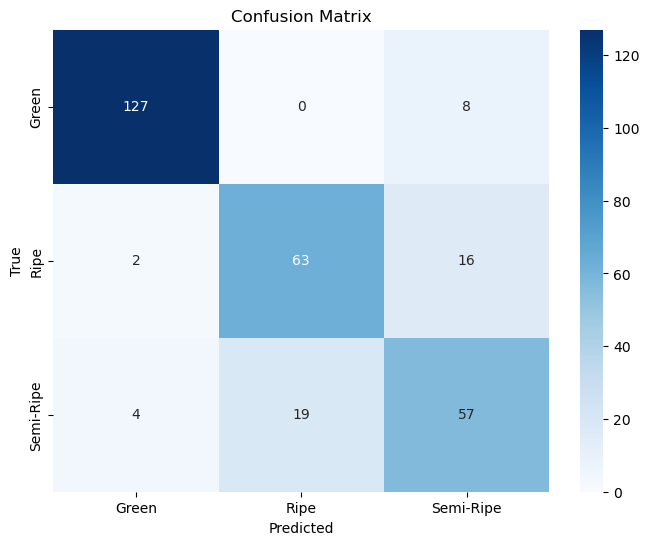
\includegraphics[width=0.5\textwidth]{kNN confusion matrix}
	\caption{Ripeness Confusion Matrix using kNN}
	\label{fig:ripeness_confusion_matrix_knn_fig}
\end{figure}

\begin{table}[htbp]
	\centering
	\begin{tabular}{c|c|c|c|c}
		\hline
		\textbf{ } & \textbf{Precision} & \textbf{Recall} & \textbf{F1} & \textbf{Support} \\
		\hline
		Green & 0.96 & 0.76 & 0.85 & 135 \\
		\hline
		Yellow Green & 0.75 & 0.30 & 0.42 & 81 \\
		\hline
		Yellow & 0.45 & 0.88 & 0.59 & 80 \\
		\hline
		Accuracy &  &  & 0.67 & 296 \\
		\hline
		Macro Avg & 0.72 & 0.64 & 0.62 & 296 \\
		\hline
		Weighted Avg & 0.76 & 0.67 & 0.66 & 296 \\
		\hline
	\end{tabular}
	\caption{Ripeness Classification Report using Naive Bayes}
	\label{tab:bruises_classification_report_naive_bayes}
\end{table}

\begin{figure}[!htbp]
	\centering
	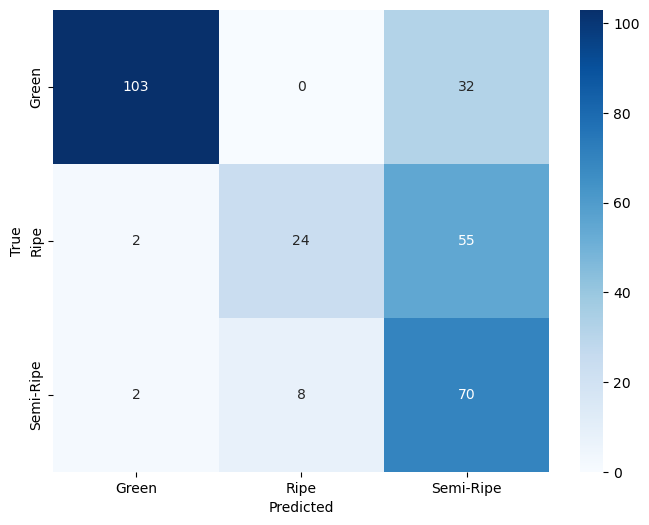
\includegraphics[width=0.5\textwidth]{naive_bayes_confusion_matrix}
	\caption{Ripeness Confusion Matrix using Naive Bayes}
	\label{fig:ripeness_confusion_matrix_nv_fig}
\end{figure}

\subsection{Bruises Classification Results} \label{sec:bruisesClassificationResults}

\begin{table}[htbp]
	\centering
	\begin{tabular}{c|c|c|c|c}
	  \hline
	  \textbf{ } & \textbf{Precision} & \textbf{Recall} & \textbf{F1} & \textbf{Support} \\
	  \hline
	  Bruised & 0.97 & 0.90 & 0.93 & 1515 \\
	  \hline
	  Not Bruised & 0.88 & 0.97 & 0.92 & 1146 \\
	  \hline
	  Accuracy &  &  & 0.93 & 2661 \\
	  \hline
	  Macro Avg & 0.93 & 0.93 & 0.93 & 2661 \\
	  \hline
	  Weighted Avg & 0.93 & 0.93 & 0.93 & 2661 \\
	  \hline
	\end{tabular}
	\caption{Bruises Classification Report using CNN}
	\label{tab:bruises_classification_report}
\end{table}

\begin{figure}[!htbp]
	\centering
	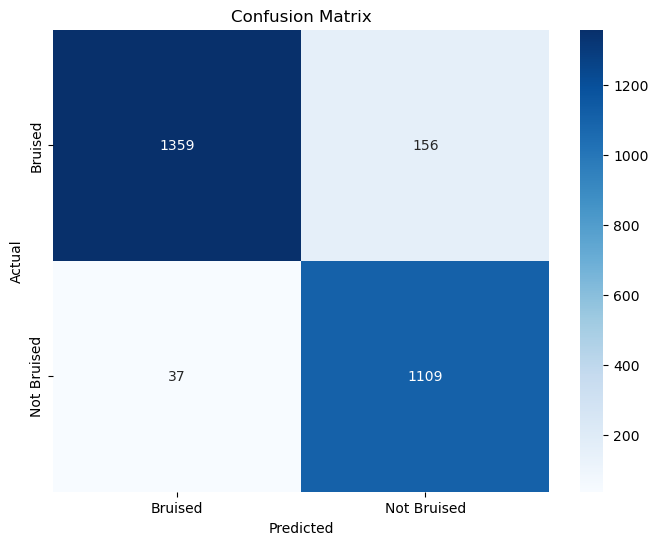
\includegraphics[width=0.5\textwidth]{bruises_confusion_matrix}
	\caption{Bruises Confusion Matrix using CNN}
	\label{fig:bruises_confusion_matrix_fig}
\end{figure}

\begin{table}[htbp]
	\centering
	\begin{tabular}{c|c}
	  \hline
	  \textbf{Metrics} & \textbf{Results} \\
	  \hline
	  Precision & 0.9318 \\
	  \hline
	  Recall & 0.9275 \\
	  \hline
	  F1 Score &  0.9278 \\
	  \hline
	\end{tabular}
	\caption{Summarized Classification Report using CNN}
	\label{tab:sum_bruises_classification_report}
\end{table}


\section{Size Determination Results} \label{sec:sizeDeterminationResults}

\section{User Priority Formula} \label{sec:userPriorityFormula}
\gls{not:bprio} and \gls{not:rprio} and \gls{not:sprio} are the \gls{User Priority-Based Grading} for bruises, ripeness, and size of the Carabao mango. 
Furthermore, \gls{not:bpred} and \gls{not:rpred} and \gls{not:spred} are the machine learning's predictions for bruises, ripeness, and size of the Carabao mango.
The formula for the user priority is given by:
\begin{equation}
	\label{eq:userPriority}
	\text{User Priority} = \ensuremath{b \left( P \right)  B\left( P \right) + r \left( P \right) R\left( P \right) + s \left( P \right) S\left( P \right)}
\end{equation}


\section{Physical Prototype} \label{sec:physicalPrototype}

Add pictures of the hardware prototype here with description

\begin{figure}[!htbp]
	\centering
	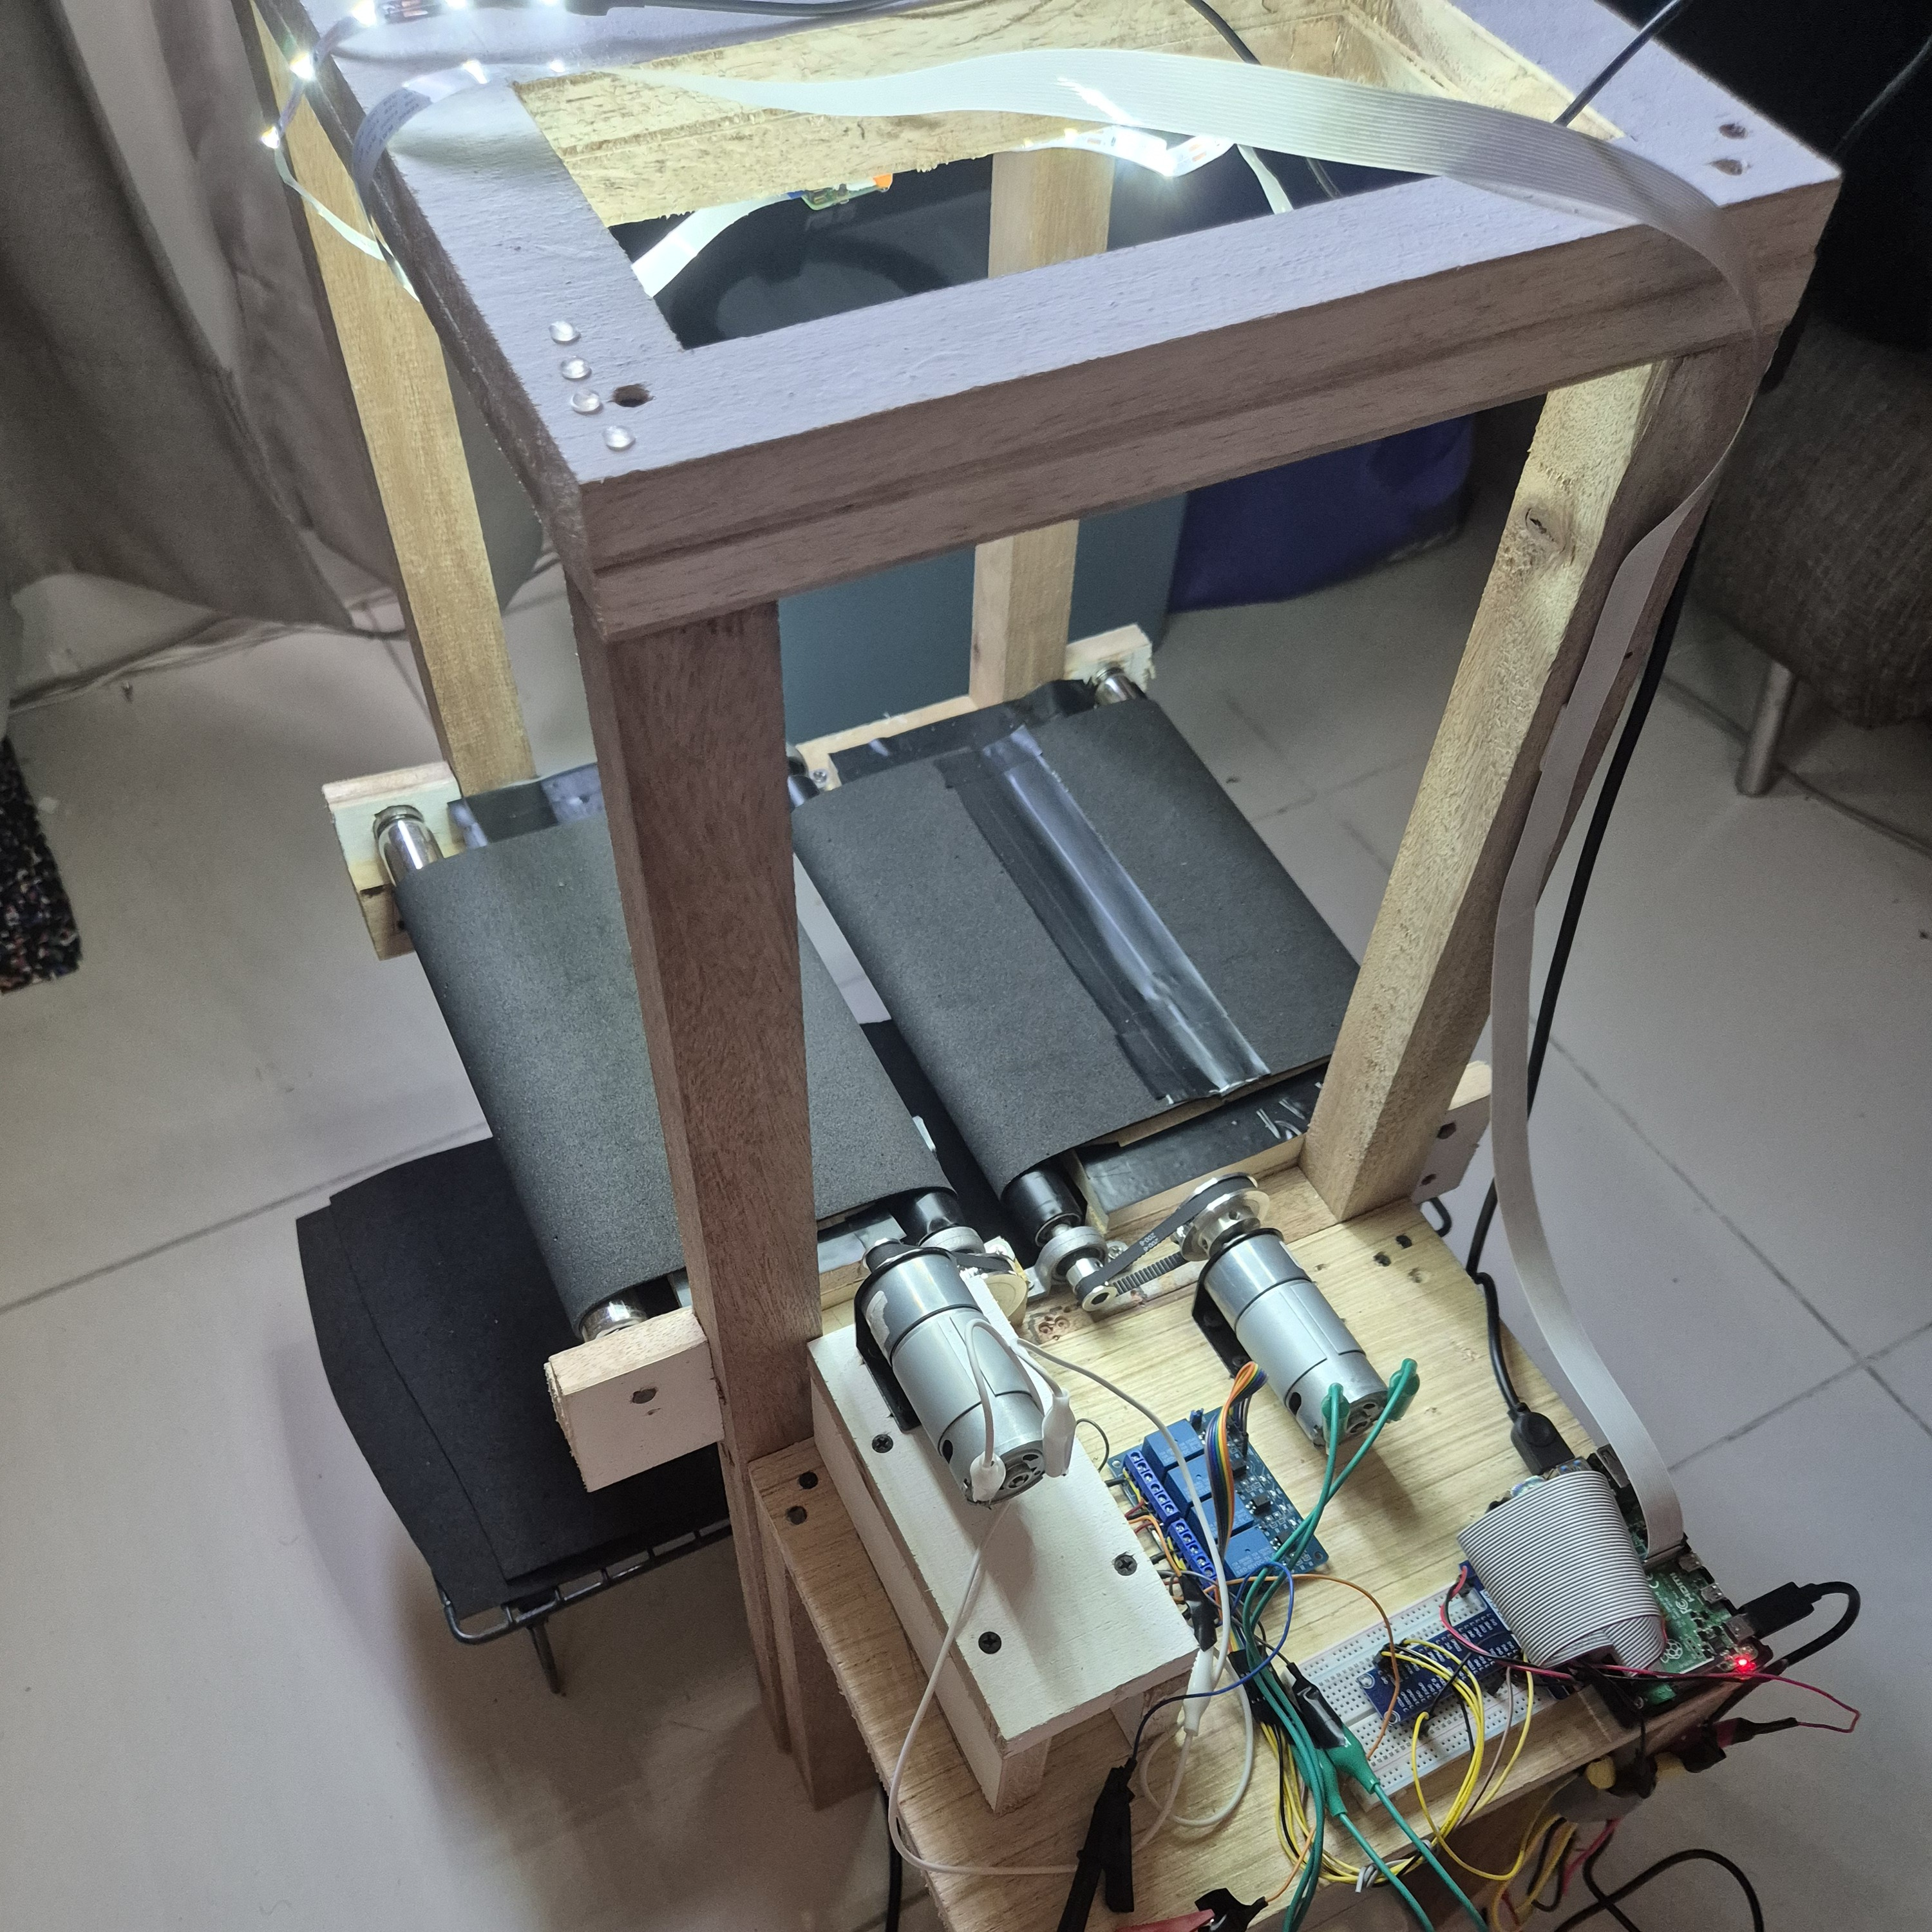
\includegraphics[width=0.5\textwidth]{top_view}
	\caption{Prototype Top View}
	\label{fig:top_view_fig}
\end{figure}

\begin{figure}[!htbp]
	\centering
	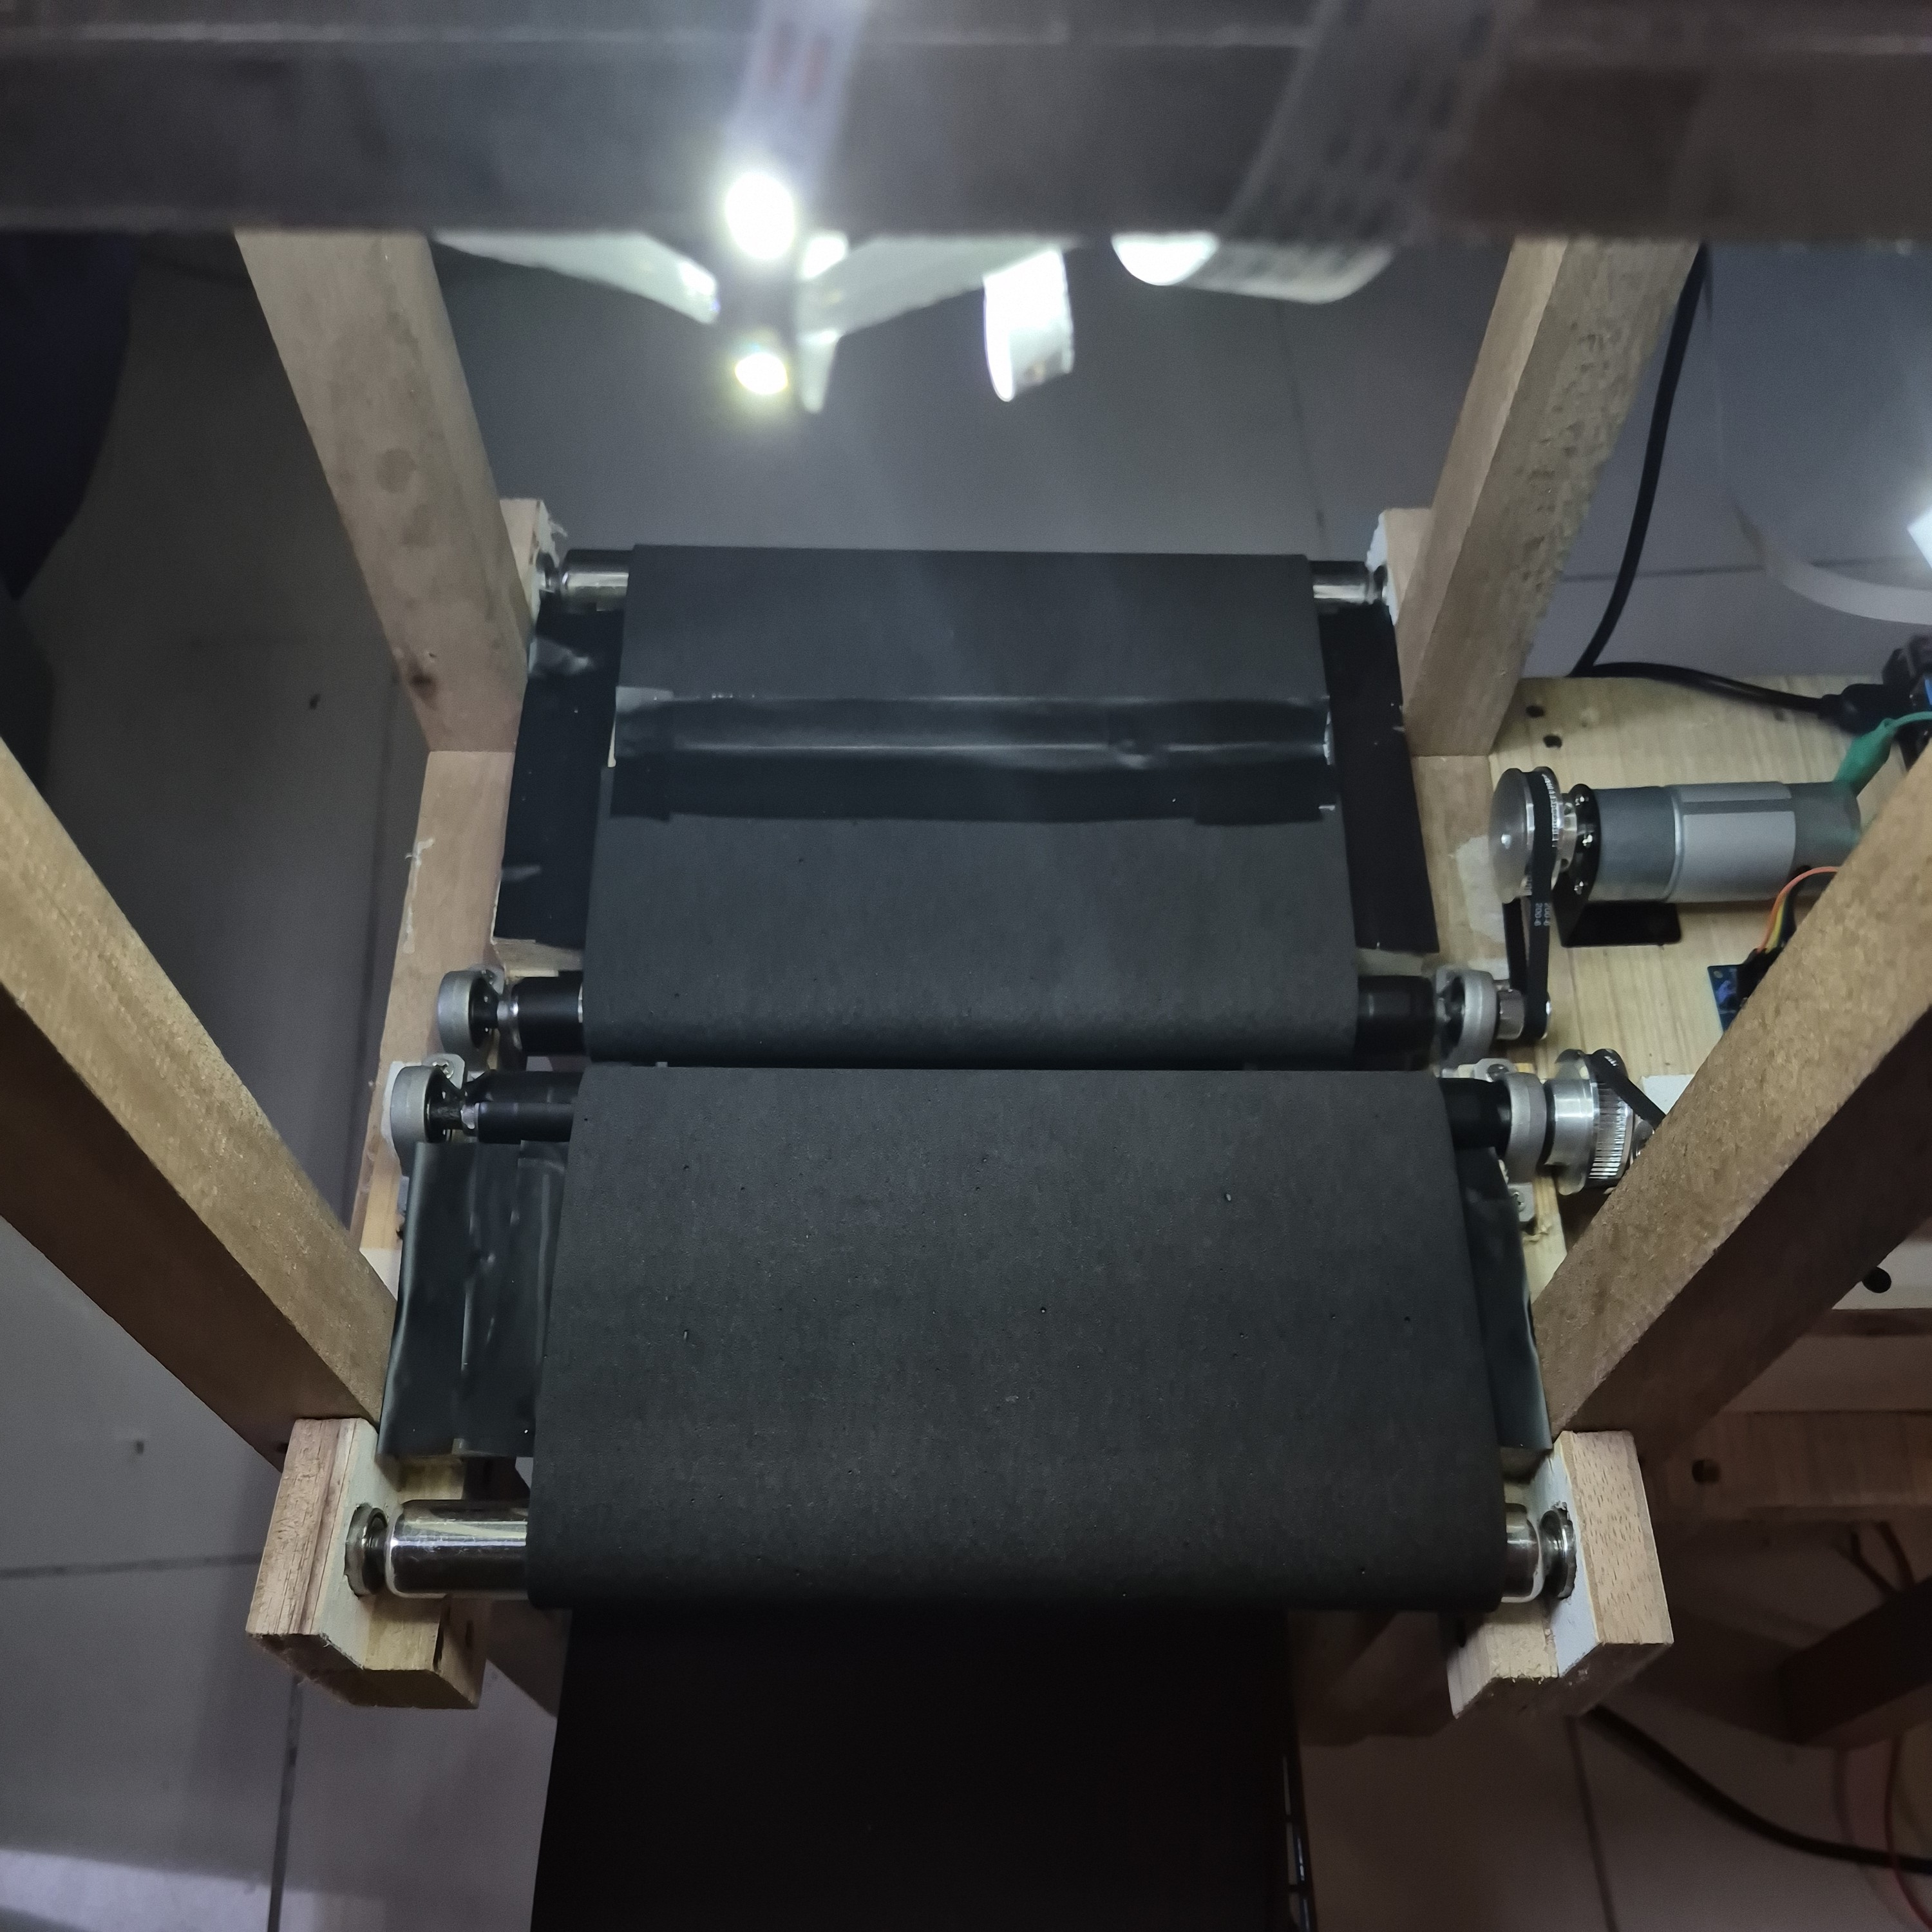
\includegraphics[width=0.5\textwidth]{side1}
	\caption{Entrance Conveyor Belt View}
	\label{fig:side1_fig}
\end{figure}

\begin{figure}[!htbp]
	\centering
	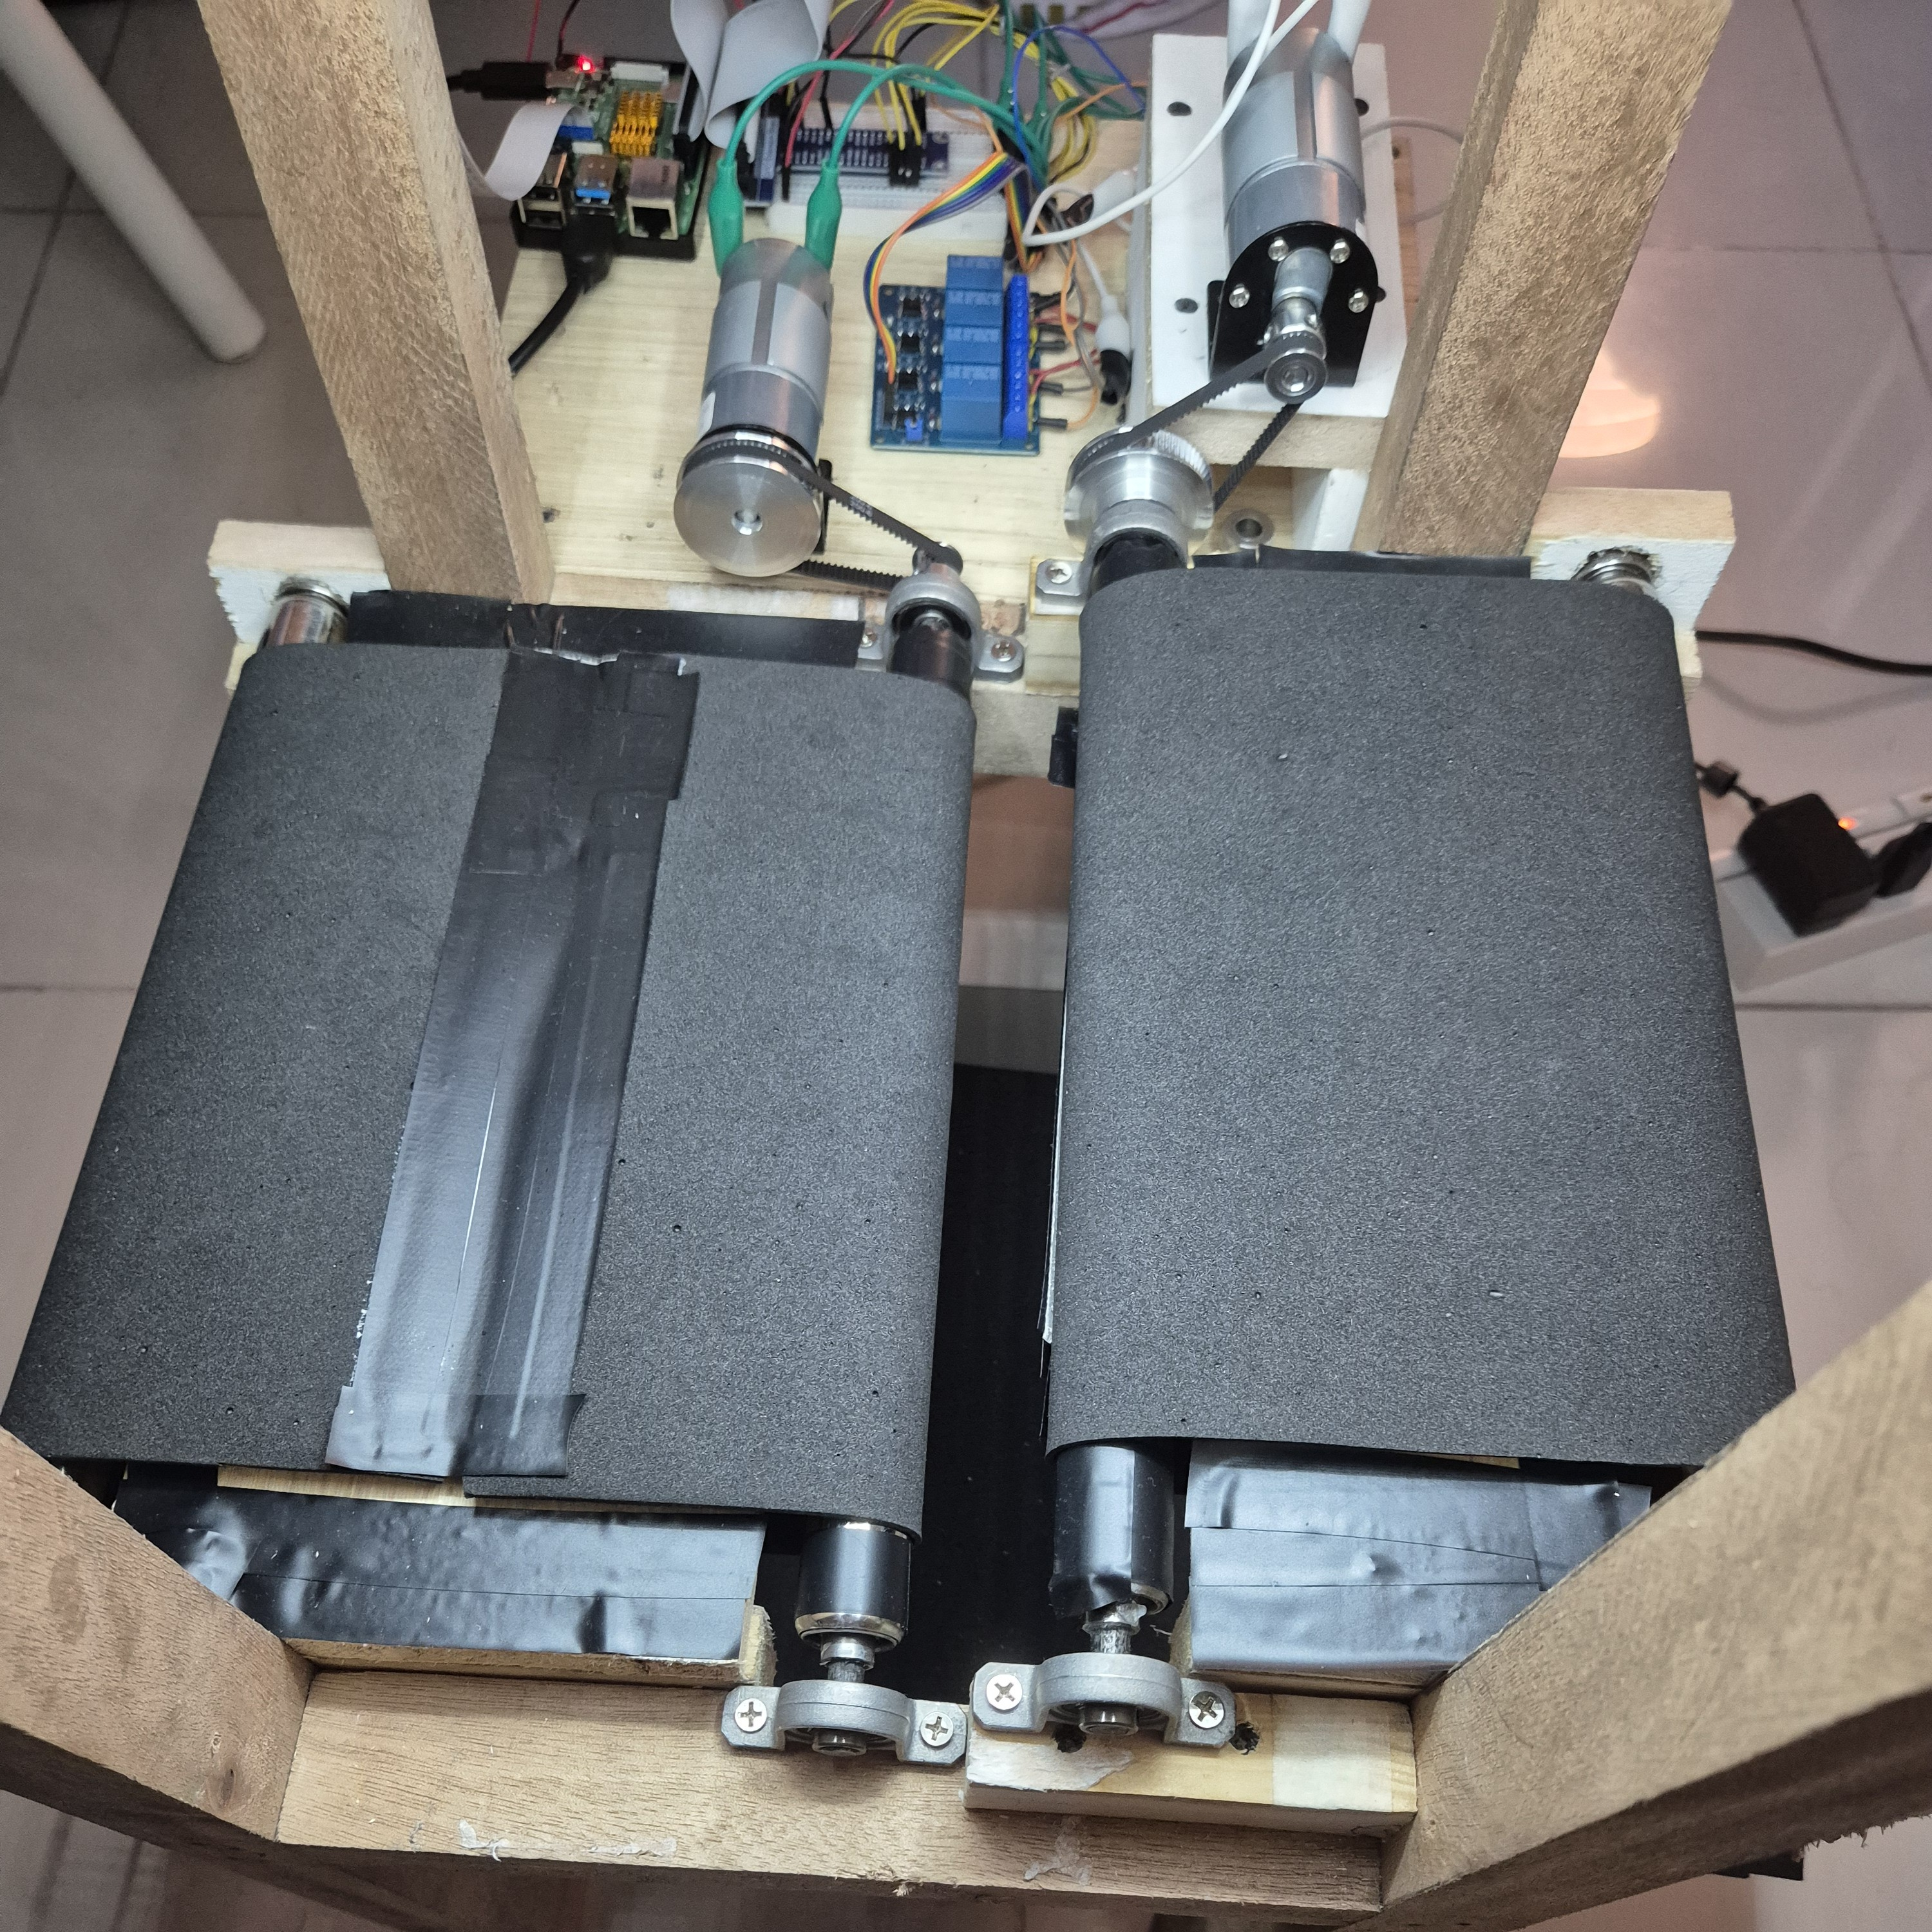
\includegraphics[width=0.5\textwidth]{side2}
	\caption{Side Conveyor Belt View}
	\label{fig:side2_fig}
\end{figure}

\begin{figure}[!htbp]
	\centering
	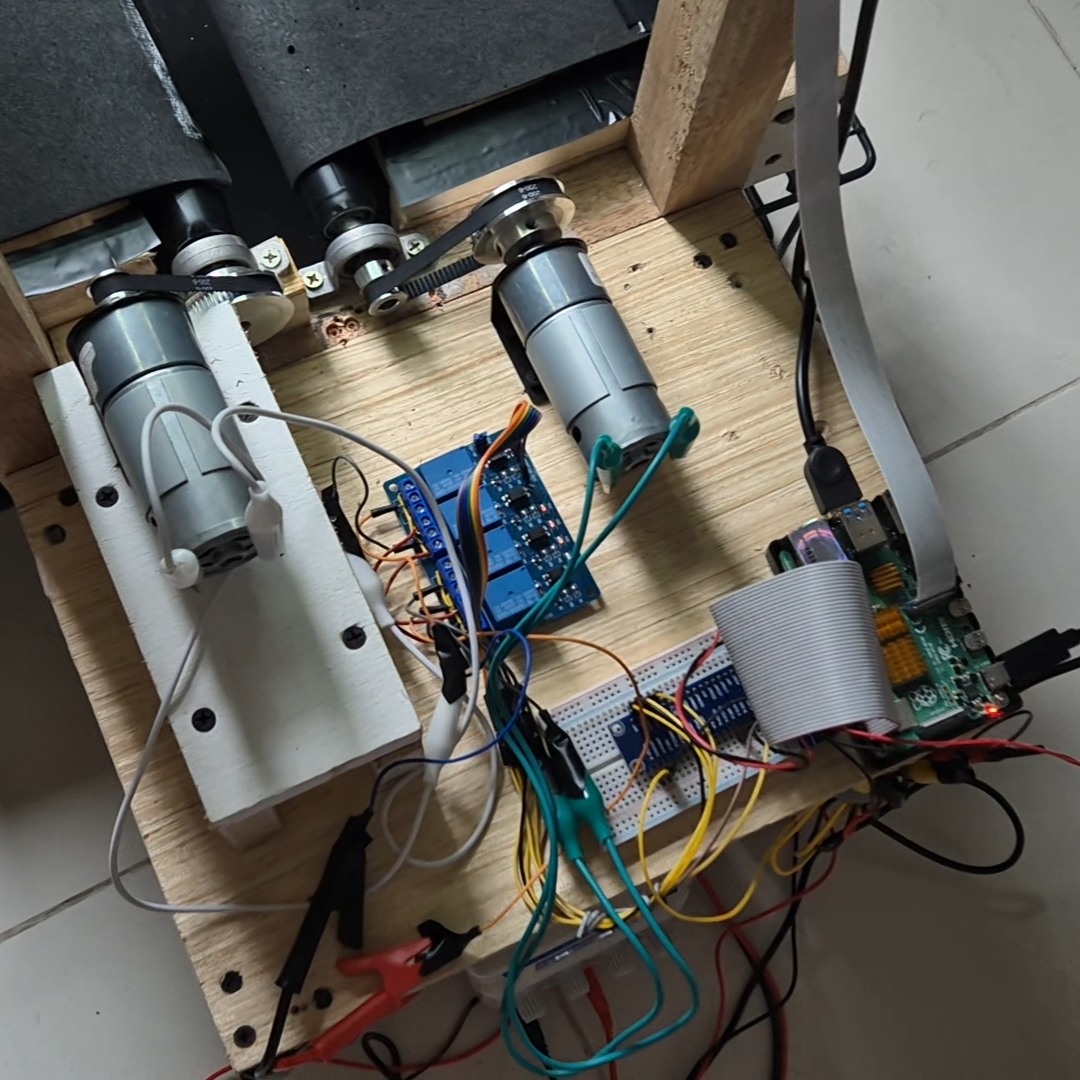
\includegraphics[width=0.5\textwidth]{schematic1}
	\caption{Prototype Main Hardware}
	\label{fig:main_hardware_fig}
\end{figure}

\begin{figure}[!htbp]
	\centering
	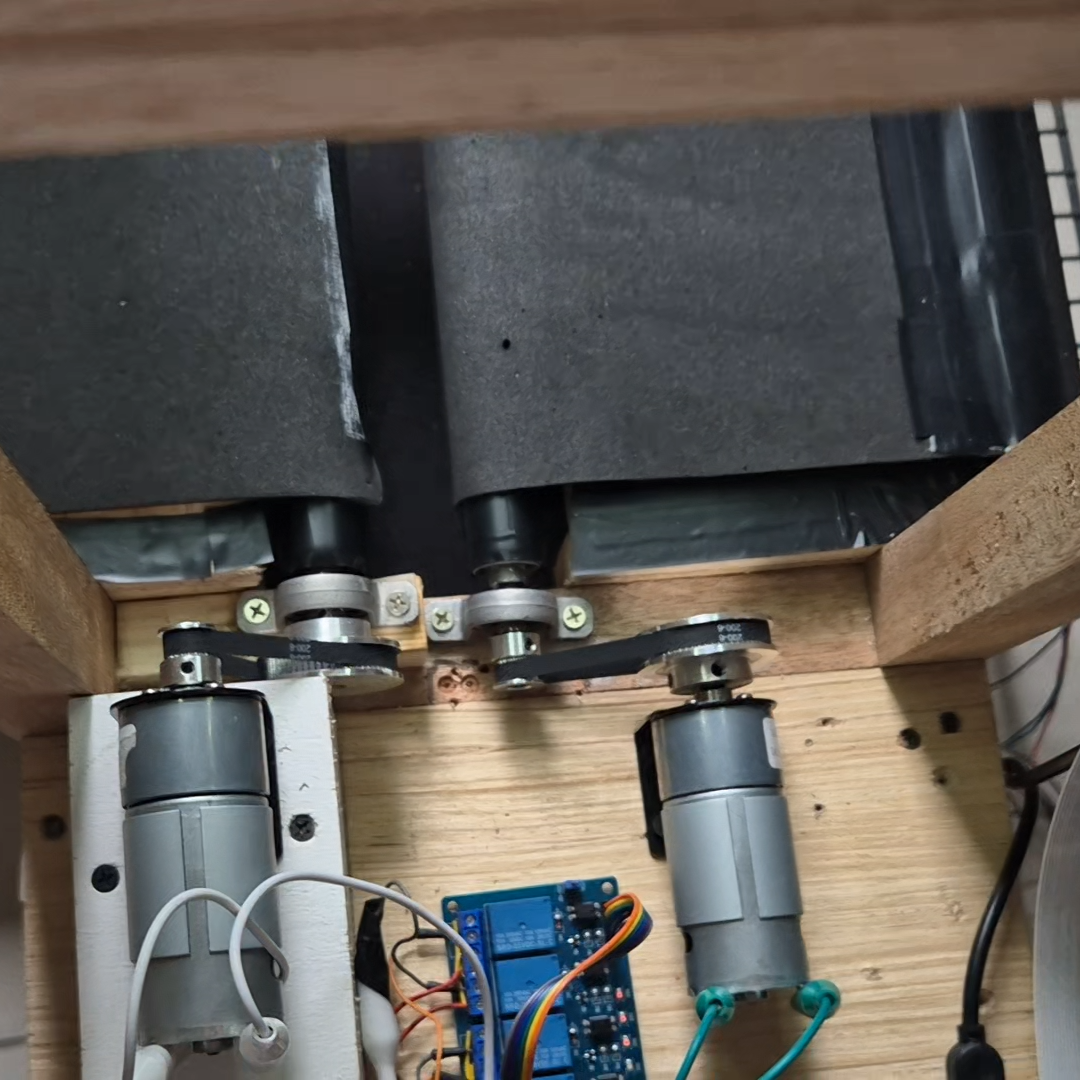
\includegraphics[width=0.5\textwidth]{DC_Motor_Pulley}
	\caption{DC Motor and Pulley}
	\label{fig:dc_motor_pulley_fig}
\end{figure}

\begin{figure}[!htbp]
	\centering
	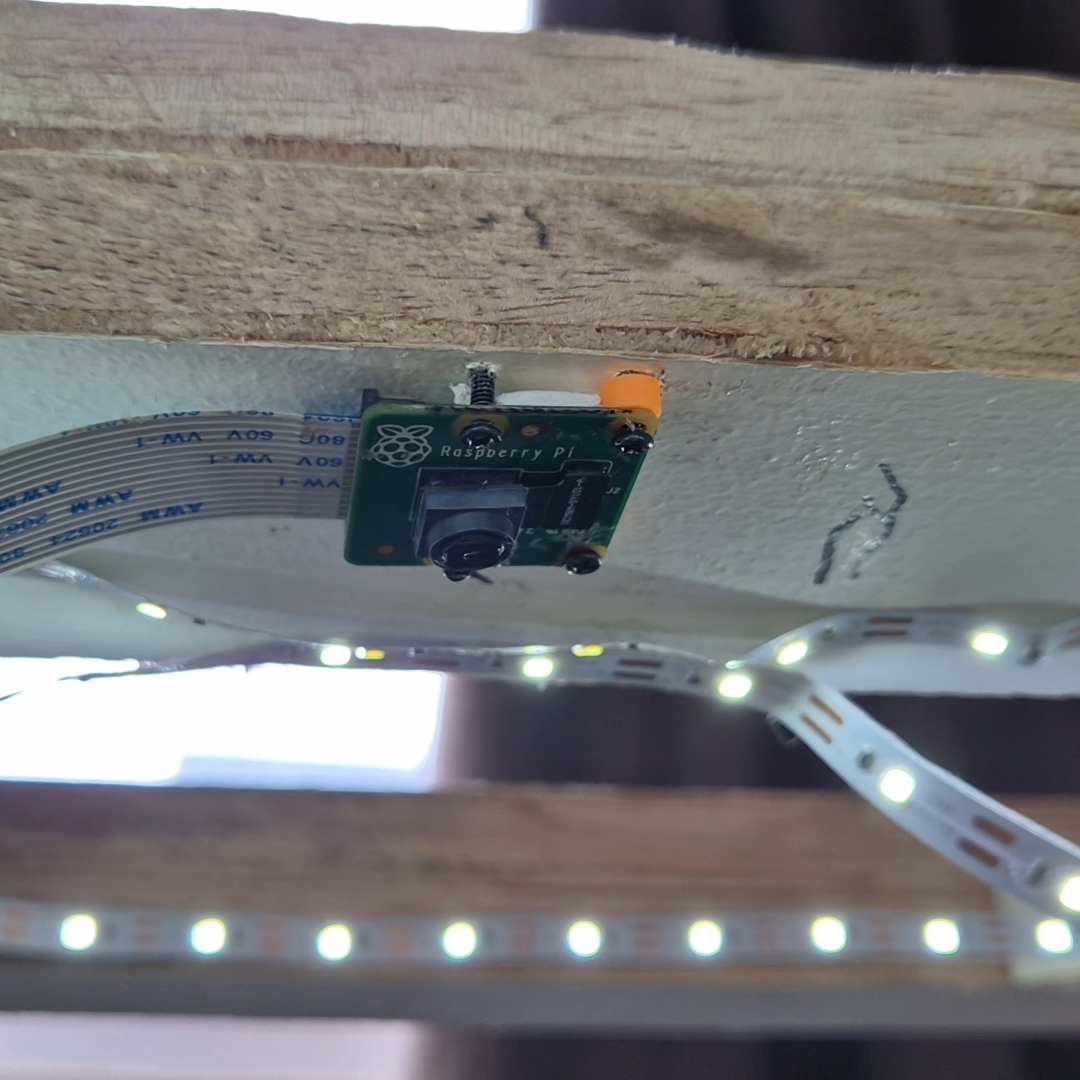
\includegraphics[width=0.5\textwidth]{camera}
	\caption{LED Lights and Camera Module}
	\label{fig:camera_fig_results}
\end{figure}

\section{Software Application}

Show the raspberry pi app UI and demonstrate it here 

\begin{figure}[!htbp]
	\centering
	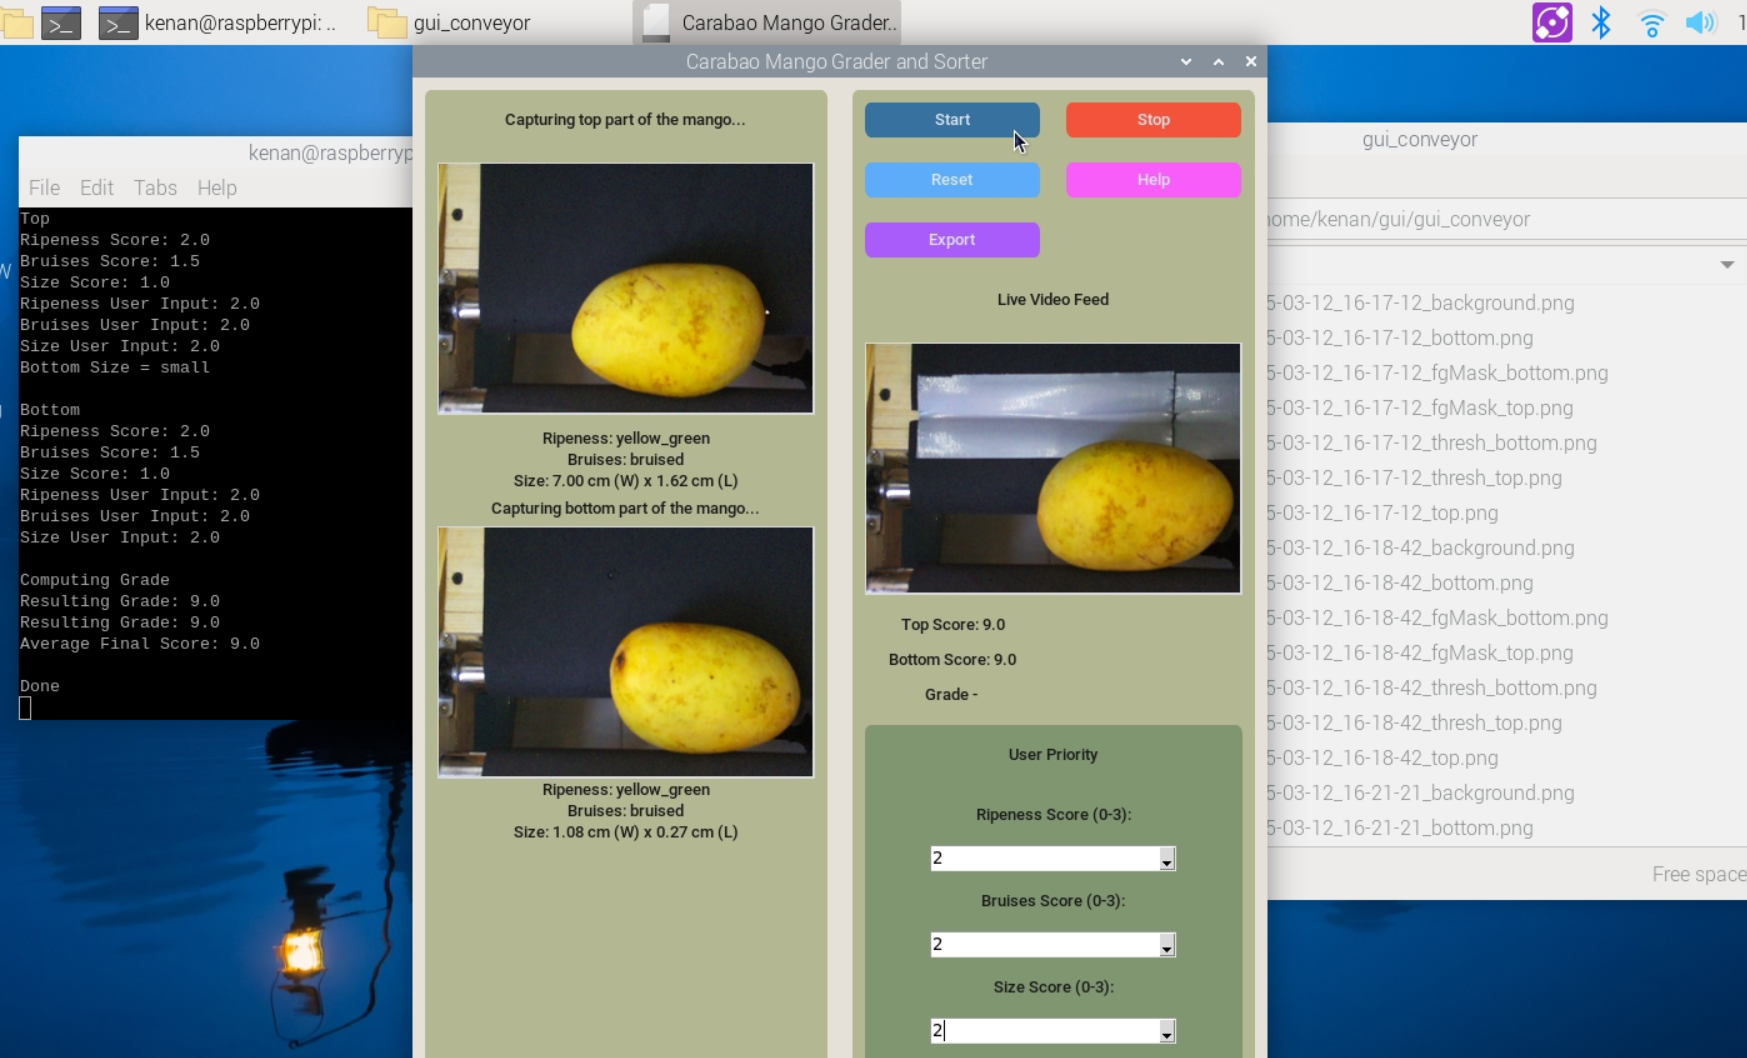
\includegraphics[width=0.9\textwidth]{UI_v1}
	\caption{Raspberry Pi App UI Version 1}
	\label{fig:app_v1_fig}
\end{figure}

\begin{figure}[!htbp]
	\centering
	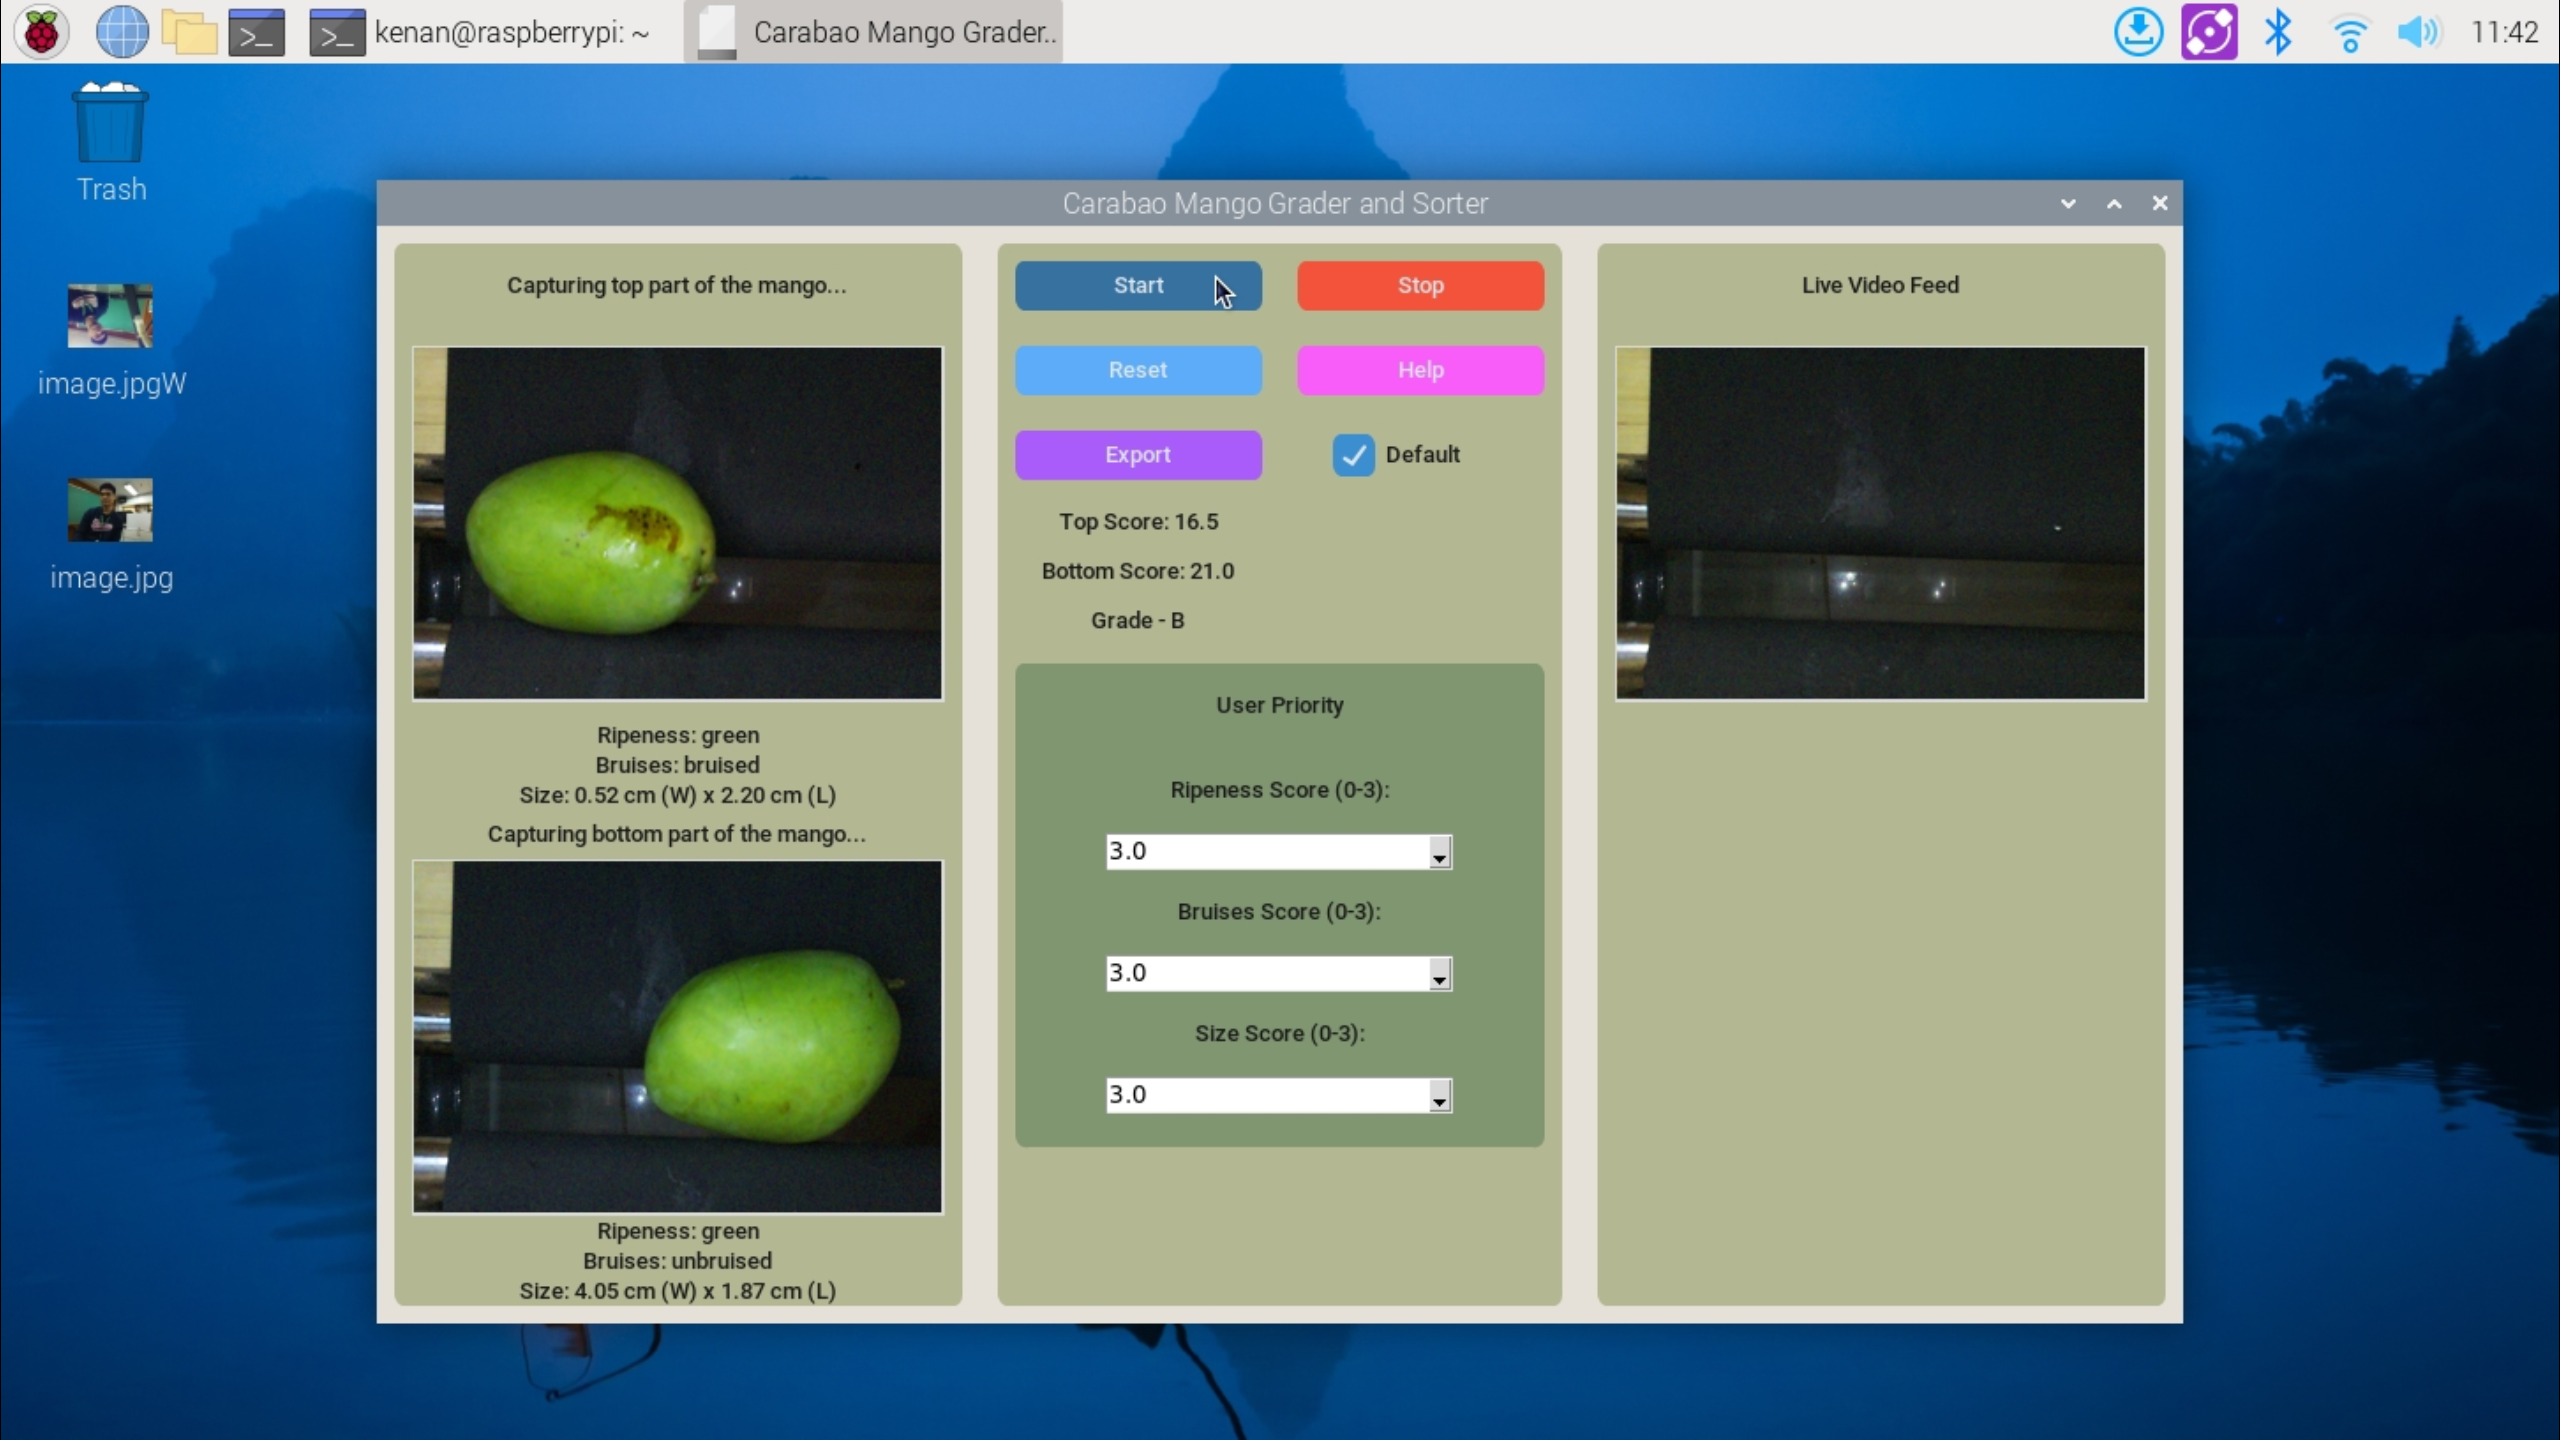
\includegraphics[width=0.9\textwidth]{UI_v2}
	\caption{Raspberry Pi App UI Version 2}
	\label{fig:app_v2_fig}
\end{figure}

\begin{figure}[!htbp]
	\centering
	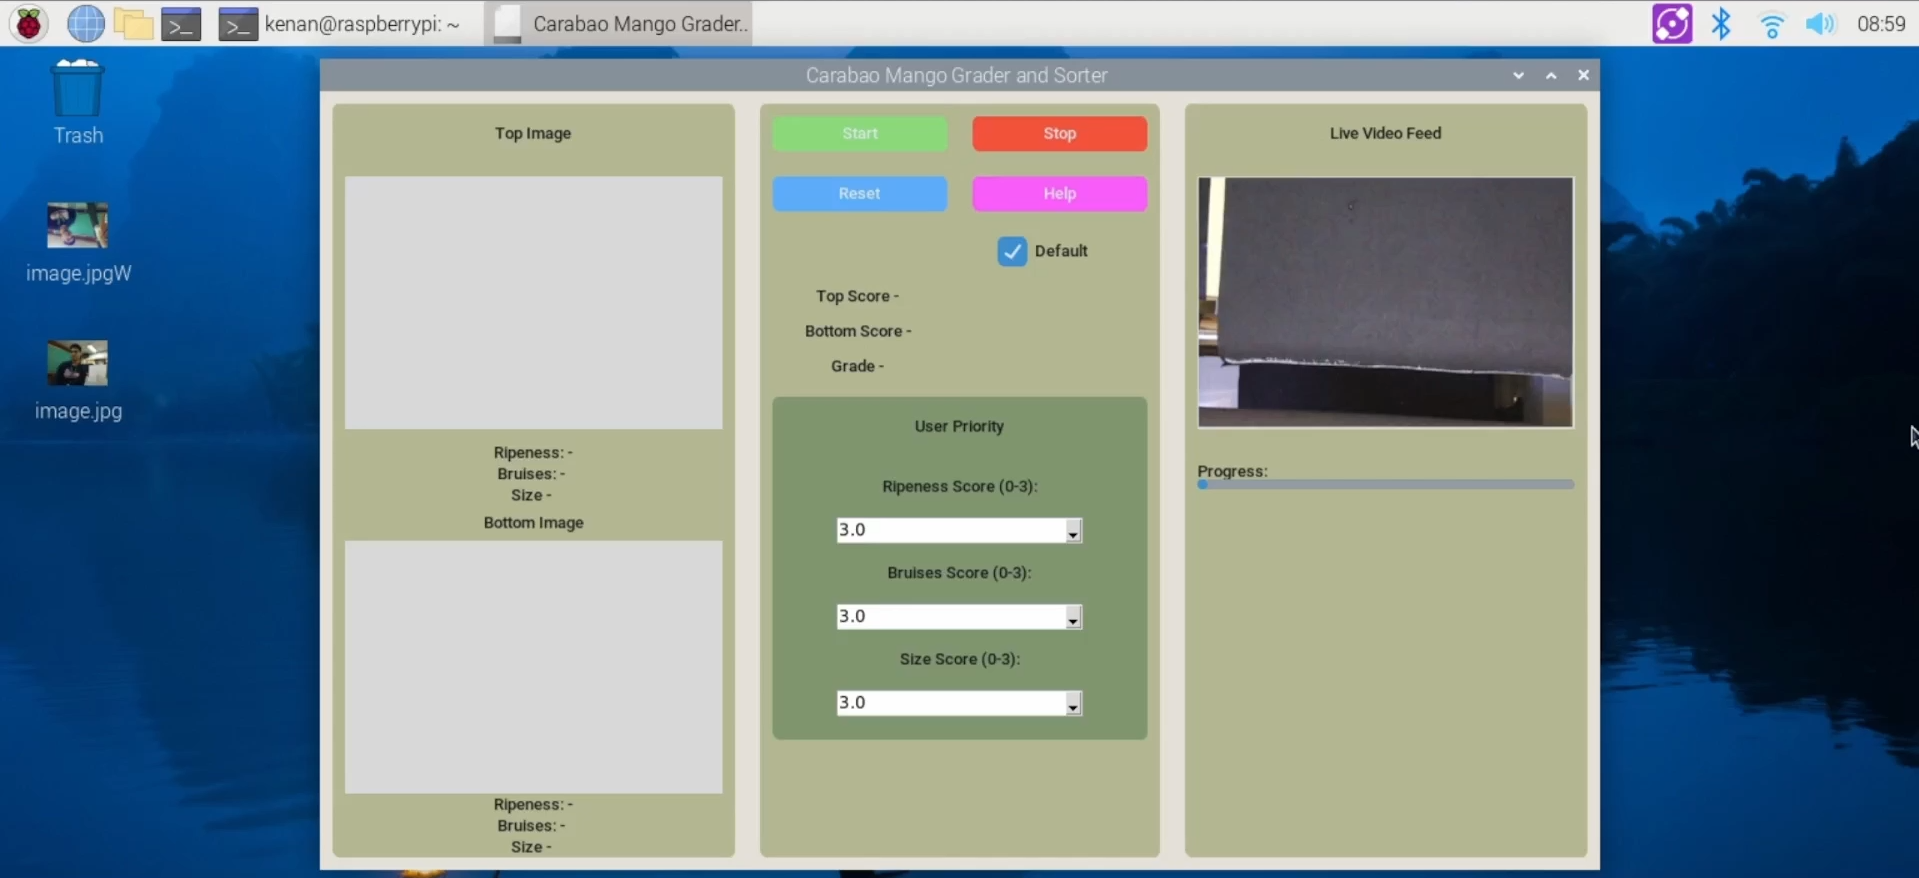
\includegraphics[width=0.9\textwidth]{UI_v3}
	\caption{Raspberry Pi App UI Version 3}
	\label{fig:app_v3_fig}
\end{figure}

\section{Summary} \label{sec:summary_results_and_discussions}

Provide the gist of this chapter such that it reflects the contents and the message.